\begin{figure}[t]
\centering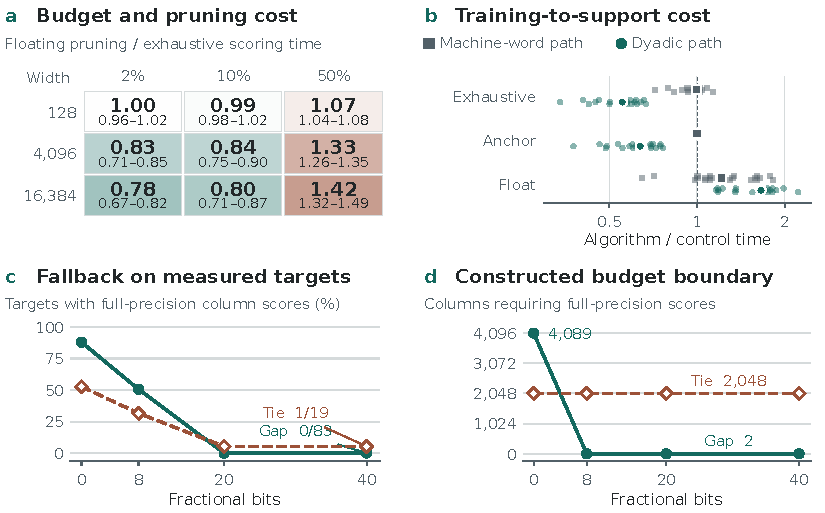
\includegraphics[width=\linewidth]{figures/cost-frontier.pdf}
\caption{(a) Floating pruning/exhaustive scoring time across 12 matrices per width and budget. Entries show medians and interquartile ranges. (b) Original 10\% training-to-support timings before tightening the bounds for silent columns. Pale marks show minPI/comparator ratios of five-call medians. Large marks give the median over 21 panels per path. (c) Fraction of targets requiring any full-precision score on six selected matrices. At 40 bits these counts are 0/83 positive gaps and 1/19 ties. (d) Number of individual columns rescored on two 4,096-column constructions at $K=\{0,4,16\}$ and $h=1$.}
\label{fig:work}
\end{figure}
